%%% CSE 4317 DDS - WORKED EXAMPLE (Full-Stack Web App). Follows IEEE Std 1016-2009.
\documentclass[11pt,letterpaper]{article}
\usepackage[margin=1.0in]{geometry}
\usepackage[T1]{fontenc}\usepackage[bitstream-charter]{mathdesign}\usepackage[latin1]{inputenc}
\usepackage{amsmath}\usepackage{xcolor}\usepackage{cite}\usepackage{hyphenat}
\usepackage{graphicx}\usepackage{float}\usepackage{subfigure}\usepackage{sectsty}
\usepackage[compact]{titlesec}\usepackage[tablegrid]{vhistory}\usepackage{pbox}\usepackage{longtable}
\allsectionsfont{\color{accentcolor}\scshape\selectfont}
\definecolor{accentcolor}{rgb}{0.0,0.0,0.5}
\newcommand{\teamname}{Team Fullstack}
\newcommand{\productname}{CivicPulse Community Service-Request Dashboard}
\newcommand{\coursename}{CSE 4317: Senior Design II}
\newcommand{\semester}{Spring 2027}
\newcommand{\docname}{Detailed Design Specification}
\newcommand{\department}{Department of Computer Science \& Engineering}
\newcommand{\university}{The University of Texas at Arlington}
\newcommand{\authors}{Alan Turing \\ Grace Hopper \\ John Von Neumann \\ Ada Lovelace \\ Charles Babbage}
\usepackage{fancyhdr}\pagestyle{fancy}\usepackage{lastpage}
\lhead{}\chead{}\rhead{}\lfoot{\footnotesize \teamname \ - \semester}\cfoot{}
\rfoot{\footnotesize page \thepage\ of \pageref{LastPage}}
\renewcommand{\headrulewidth}{0.0pt}\renewcommand{\footrulewidth}{0.4pt}
\usepackage[runin]{abstract}\abslabeldelim{\quad}\setlength{\abstitleskip}{-10pt}
\renewcommand{\abstractname}{}\renewcommand{\abstracttextfont}{\color{accentcolor} \small \slshape}

\begin{document}
{\centering \huge \color{accentcolor} \sc \textbf{\department \\ \university} \par}
\vspace{1 in}
{\centering \huge \color{accentcolor} \sc \textbf{\docname \\ \coursename \\ \semester} \par}
\vspace{0.5 in}
\begin{figure}[h!]\centering
\includegraphics[width=0.60\textwidth]{images/test_image}\end{figure}
\vspace{0.5 in}
{\centering \huge \color{accentcolor} \sc \textbf{\teamname \\ \productname} \par}
\vspace{0.5 in}{\centering \large \sc \textbf{\authors} \par}
\newpage
\begin{versionhistory}
  \vhEntry{0.1}{01.20.2027}{JVN}{document creation}
  \vhEntry{1.0}{02.05.2027}{AT|GH|CB}{official release}
\end{versionhistory}
\newpage\setcounter{tocdepth}{2}\tableofcontents\newpage

\section{Introduction}
Implementation-level design of \productname\ as an IEEE 1016-2009 \cite{IEEE1016}
Software Design Description, building on the SRS and ADS (tiers X/Y/Z).

\section{Design Stakeholders \& Concerns}
Implementers, integrators, testers, city IT (maintainers); concerns of composition,
data, interfaces, state, algorithms, and resources.

\section{Design Viewpoints}
Context, Composition, Information, Interface, Interaction \& State, Algorithm,
Resource per IEEE 1016; omitted where not applicable.

\section{System Overview}
\begin{figure}[h!]\centering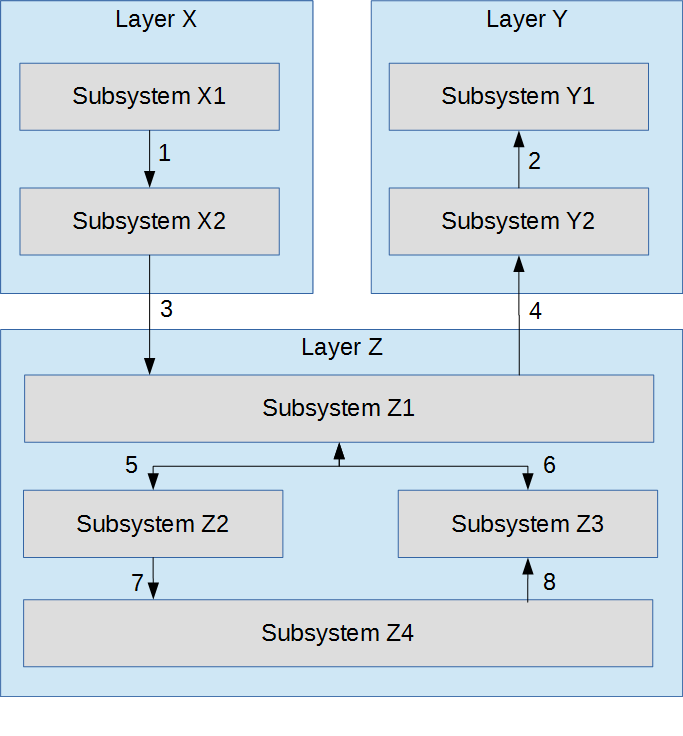
\includegraphics[width=0.9\textwidth]{images/data_flow}
\caption{Three-tier deployment carried forward from the ADS}\end{figure}
Frontend: React/TypeScript SPAs served by a CDN/reverse proxy. Backend: containerized
Node/TypeScript (NestJS) API. Data: managed PostgreSQL + PostGIS and object storage.

\section{X Layer Subsystems --- Presentation}
\subsection{Layer Resources}
\textbf{Deps:} React, TypeScript, a map library; \textbf{Language:} TypeScript.
\subsection{X.ResidentPortal \& X.StaffDashboard}
\textbf{Composition:} SPA route modules (submit, track, dashboard, request detail).
\textbf{Interface (\#01):} calls the REST API; renders map via EI-02. \textbf{State:}
client form/query state; auth token held in memory for staff. \textbf{Interaction:}
optimistic status updates with server confirmation. \textbf{Rationale:} SPA split
enables responsive/accessible UI (US-01) over the stateless API (AD-01).

\section{Y Layer Subsystems --- Application}
\subsection{Layer Resources}
\textbf{Deps:} NestJS, an OIDC client, an ORM, an SMTP client; \textbf{Language:}
TypeScript.
\subsection{Y.APIGateway}
\textbf{Interface (\#02):} REST; validates OIDC access tokens (EI-01) and enforces
RBAC middleware (SE-01). \textbf{Algorithm:} per-route role guard; deny by default.
\subsection{Y.RequestService}
\textbf{Information:} \texttt{Request\{id, category, description, geom(Point),
photo\_ref, status, priority, assignee, history[]\}}. \textbf{Interface:} CRUD +
triage/assign endpoints. \textbf{State:} status machine
\texttt{NEW$\rightarrow$TRIAGED$\rightarrow$ASSIGNED$\rightarrow$IN\_PROGRESS
$\rightarrow$RESOLVED$\rightarrow$CLOSED}. \textbf{Algorithm (FR-05):} on create,
\texttt{ST\_DWithin} PostGIS query for same-category requests within radius/time;
flag matches. \textbf{Rationale:} PostGIS does the spatial work natively.
\subsection{Y.NotificationService}
On status change, render a template and send via SMTP (FR-04); failures retried and
logged (MS-01).

\section{Z Layer Subsystems --- Data}
\subsection{Layer Resources}
\textbf{Tech:} PostgreSQL + PostGIS; object storage; \textbf{Language:} SQL/migrations.
\subsection{Z.Datastore}
\textbf{Information:} normalized tables \texttt{requests, users, assignments,
status\_history, audit}; spatial index on \texttt{geom}. \textbf{Interface:} ORM +
migrations. \subsection{Z.Integrations}
Adapters for geocoding (EI-02) and SMTP behind interfaces so providers can be
swapped without touching services.

\section{Requirements Traceability}
\begin{table}[H]\begin{center}\begin{tabular}{ | p{1.6cm} | p{5cm} | p{3.4cm} | p{1.6cm} |}\hline
\textbf{Req} & \textbf{Requirement (abbrev.)} & \textbf{Component} & \textbf{Iface} \\ \hline
FR-01/02 & Submit/track & X.ResidentPortal, Y.RequestService & \#01 \\ \hline
FR-03 & Triage/assign & Y.RequestService & \#02 \\ \hline
FR-04 & Status/notify & Y.NotificationService & --- \\ \hline
FR-05 & Duplicates & Y.RequestService, Z.Datastore & --- \\ \hline
SE-01 & RBAC+TLS & Y.APIGateway & \#02 \\ \hline
\end{tabular}\end{center}\end{table}

\section{Appendix A}
Database schema, OpenAPI specification, and infrastructure-as-code are attached to
the closeout package.

\bibliographystyle{reference/IEEEtran_custom}
\bibliography{reference/refs}{}
\end{document}
